\documentclass[12pt]{article}

\usepackage{fullpage}
\usepackage{multicol,multirow}
\usepackage{tabularx}
\usepackage{ulem}
\usepackage[utf8]{inputenc}
\usepackage[russian]{babel}
\usepackage{listings}
\usepackage{hyperref}
\usepackage{graphicx}
\usepackage{amsmath}
\usepackage{xcolor}
\DeclareGraphicsExtensions{.png}


\begin{document}

\section*{Лабораторная работа №\,3 по курсу криптографии}

Выполнила студентка группы М8О-307Б \textit{Безлуцкая Елизавета}.

\subsection*{Условие}
\begin{enumerate}
\item Строку в которой записано своё ФИО подать на вход в хеш-функцию ГОСТ Р 34.11-2012 (Стрибог). Младшие 4 бита выхода интерпретировать как число, которое в дальнейшем будет номером варианта. Процесс выбора варианта требуется отразить в отчёте.
\item Программно реализовать один из алгоритмов функции хеширования в соответствии с номером варианта. Алгоритм содержит в себе несколько раундов.
\item Модифицировать оригинальный алгоритм таким образом, чтобы количество раундов было настраиваемым параметром программы. в этом случае новый алгоритм не будет являться стандартом, но будет интересен для исследования.
\item Применить подходы дифференциального криптоанализа к полученным алгоритмам с разным числом раундов.
\item Построить график зависимости количества раундов и возможности различения отдельных бит при количестве раундов 1,2,3,4,5,... .
\item Сделать выводы.
\end{enumerate}

\subsection*{Метод решения}
Выбор варианта произведен с помощью библиотеки pygost:\\
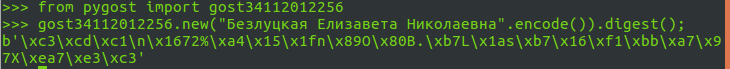
\includegraphics[width=\linewidth]{images/var.png}\\

\textbf{Вариант 3: BLAKE}
Для реализации я выбрала BLAKE-256. Функция работает следующим образом:\\

\textbf{1 этап: padding}\\
Сообщение дополняется функцией \textbf{padding} данными для кратности 512 битам (64 байтам): сначала -- битами, так, что его длина становится по модулю 512 равной 447: сначала добавляется 1, затем необходимое количество нолей. После этого прибавляется ещё одна 1 и 64-битное представление длины сообщения l от старшего бита к младшему. Таким образом, длина сообщения становится кратной 512. \textbf{Padding} гарантирует, что длина сообщения станет кратной 512 битам.\\

\newpage

\textbf{2 этап: compress}\\

Затем, блок за блоком, сообщение обрабатывает функция сжатия \textbf{compression}.\\
Она принимает на вход:
\begin{itemize}
\item Переменные цепочки \textbf{h = h0,...,h7} (8 слов);
\item Блок сообщения \textbf{m = m0,...,m15};
\item Значение соли \textbf{s = s0,...,s3};
\item Значение счётчика \textbf{t = t0,t1}.
\end{itemize}

Таким образом, на вход ей подаётся 30 слов (8+16+4+2=30, 30*4 = 120 байт = 960 бит). Возвращает функция сжатия только новое значение переменных цепочки: \textbf{h' = h'0,...,h'7}.\\

\textbf{Константы}\\
Существуют начальные константы\\

INITIAL VALUES (IV):\\
IV0 = 6A09E667 \quad IV1 = BB67AE85\\
IV2 = 3C6EF372 \quad IV3 = A54FF53A\\
IV4 = 510E527F \quad IV5 = 9B05688C\\
IV6 = 1F83D9AB \quad IV7 = 5BE0CD19\\

16 констант (Первые цифры числа пи):\\
c0  = 243F6A88 \quad c1  = 85A308D3\\
c2  = 13198A2E \quad c3  = 03707344\\
c4  = A4093822 \quad c5  = 299F31D0\\
c6  = 082EFA98 \quad c7  = EC4E6C89\\
c8  = 452821E6 \quad c9  = 38D01377\\
c10 = BE5466CF \quad c11 = 34E90C6C\\
c12 = C0AC29B7 \quad c13 = C97C50DD\\
c14 = 3F84D5B5 \quad c15 = B5470917\\

перестановки {0,...,15} (используются во всех функциях BLAKE):\\
$
\sigma = 
\left[
\begin{array}{*{16}c}
  0 &  1 &  2 &  3 &  4 &  5 &  6 &  7 &  8 &  9 & 10 & 11 & 12 & 13 & 14 & 15\\
 14 & 10 &  4 &  8 &  9 & 15 & 13 &  6 &  1 & 12 &  0 &  2 & 11 &  7 &  5 &  3\\
 11 &  8 & 12 &  0 &  5 &  2 & 15 & 13 & 10 & 14 &  3 &  6 &  7 &  1 &  9 &  4\\
  7 &  9 &  3 &  1 & 13 & 12 & 11 & 14 &  2 &  6 &  5 & 10 &  4 &  0 & 15 &  8\\
  9 &  0 &  5 &  7 &  2 &  4 & 10 & 15 & 14 &  1 & 11 & 12 &  6 &  8 &  3 & 13\\
  2 & 12 &  6 & 10 &  0 & 11 &  8 &  3 &  4 & 13 &  7 &  5 & 15 & 14 &  1 &  9\\
 12 &  5 &  1 & 15 & 14 & 13 &  4 & 10 &  0 &  7 &  6 &  3 &  9 &  2 &  8 & 11\\
 13 & 11 &  7 & 14 & 12 &  1 &  3 &  9 &  5 &  0 & 15 &  4 &  8 &  6 &  2 & 10\\
  6 & 15 & 14 &  9 & 11 &  3 &  0 &  8 & 12 &  2 & 13 &  7 &  1 &  4 & 10 & 5\\
 10 &  2 &  8 &  4 &  7 &  6 &  1 &  5 & 15 & 11 &  9 & 14 &  3 & 12 & 13 & 0
 
\end{array}
\right]
$
\\

\textbf{Инициализация}\\

16 переменных, \textbf{v0,...,v15}, описывающих текущее состояние v, инициализируются начальными значениями в зависимости от входных данных и представлены в виде матрицы 4x4:\\
\[
\begin{bmatrix}
    v_{0}	& v_{1}		& v_{2} 	& v_{3} \\
    v_{4}	& v_{5} 	& v_{6}		& v_{7} \\
    v_{8}	& v_{9} 	& v_{10} 	& v_{11} \\
    v_{12}	& v_{13} 	& v_{14} 	& v_{15}
\end{bmatrix}
\leftarrow
\begin{bmatrix}
    h_{0}			   & h_{1}				& h_{2} 	         & h_{3} \\
    h_{4}			   & h_{5} 			    & h_{6}		         & h_{7} \\
    s_{0} \oplus c_{0} & s_{1} \oplus c_{1} & s_{2} \oplus c_{2} & s_{3} \oplus c_{3} \\
    t_{0} \oplus c_{4} & t_{0} \oplus c_{5}	& t_{1} \oplus c_{6} & t_{1} \oplus c_{7}
\end{bmatrix}
\]
\\

\textbf{Раундовая функция}\\

После того, как состояние \textbf{v} инициализировано, запускается серия из 14 раундов. Раунд — это операция над состоянием $v$, которая производит вычисления, разбитые на следующие блоки:\\
$$G_{0}(v_{0}, v_{4}, v_{8}, v_{12}) \quad G_{1}(v_{1}, v_{5}, v_{9}, v_{13}) \quad G_{2}(v_{2}, v_{6}, v_{10}, v_{14}) \quad G_{3}(v_{3}, v_{7}, v_{11}, v_{15})$$
$$G_{4}(v_{0}, v_{5}, v_{10}, v_{15}) \quad G_{5}(v_{1}, v_{6}, v_{11}, v_{12}) \quad G_{6}(v_{2}, v_{7}, v_{8}, v_{13}) \quad G_{7}(v_{3}, v_{4}, v_{9}, v_{14})$$\\
на r-ом раунде блок вычислений $G_{i}(a,b,c,d)$ работает следующим образом:\\
$ j \leftarrow \sigma_{r\%10}[2 \cdot i]\\
  j \leftarrow \sigma_{r\%10}[2 \cdot i + 1]\\
  a \leftarrow a + b + (m_{j} \oplus c_{k})\\
  d \leftarrow (d \oplus a) >>> 16\\
  c \leftarrow c + d\\
  b \leftarrow (b \oplus c) >>> 12\\
  a \leftarrow a + b + (m_{k} \oplus c_{j})\\
  d \leftarrow (d \oplus a) >>> 8\\
  c \leftarrow c + d\\
  b \leftarrow (b \oplus c) >>> 7$\\
  
\textbf{Последний шаг}\\

После всех раундов новое значение переменных цепочки $h'_{0},...,h'_{7}$ вычисляется из переменных $v_{0},...,v_{15}$ матрицы состояния, входных переменных $h$ и из соли $s$:\\
$
h'_{0} \leftarrow h_{0} \oplus s_{0} \oplus v_{0} \oplus v{8}\\
h'_{1} \leftarrow h_{1} \oplus s_{1} \oplus v_{1} \oplus v{9}\\
h'_{2} \leftarrow h_{2} \oplus s_{2} \oplus v_{2} \oplus v{10}\\
h'_{3} \leftarrow h_{3} \oplus s_{3} \oplus v_{3} \oplus v{11}\\
h'_{4} \leftarrow h_{4} \oplus s_{0} \oplus v_{4} \oplus v{12}\\
h'_{5} \leftarrow h_{5} \oplus s_{1} \oplus v_{5} \oplus v{13}\\
h'_{6} \leftarrow h_{6} \oplus s_{2} \oplus v_{6} \oplus v{14}\\
h'_{7} \leftarrow h_{7} \oplus s_{3} \oplus v_{7} \oplus v{15}
$\\

Реализация алгоритма отчасти была позаимствована из \url{https://www.springer.com/gp/book/9783662447567}

\subsubsection*{Исходный код}

\definecolor{mGreen}{rgb}{0,0.6,0}
\definecolor{mGray}{rgb}{0.5,0.5,0.5}
\definecolor{mPurple}{rgb}{0.58,0,0.82}
\definecolor{backgroundColour}{rgb}{0.95,0.95,0.92}

\lstdefinestyle{CStyle}{
    backgroundcolor=\color{backgroundColour},   
    commentstyle=\color{mGreen},
    keywordstyle=\color{magenta},
    numberstyle=\tiny\color{mGray},
    stringstyle=\color{mPurple},
    basicstyle=\footnotesize,
    breakatwhitespace=false,         
    breaklines=true,                 
    captionpos=b,                    
    keepspaces=true,                 
    numbers=left,                    
    numbersep=5pt,                  
    showspaces=false,                
    showstringspaces=false,
    showtabs=false,                  
    tabsize=2,
    language=C
}
 
\textbf{blake256.h}
\lstinputlisting[style=CStyle]{code/blake256.h}

\textbf{main.c}
\lstinputlisting[style=CStyle]{code/main.c}

\subsubsection*{Консоль}
\begin{lstlisting}

->blake256 ./blake 
Input message: 
Digest: 716f6e863f744b9ac22c97ec7b76ea5f5908bc5b2f67c61510bfc4751384ea7a
->blake256 ./blake 
Input message: The quick brown fox jumps over the lazy dog
Digest: 7576698ee9cad30173080678e5965916adbb11cb5245d386bf1ffda1cb26c9d7
->blake256 ./blake
Input message: BLAKE
Digest: 07663e00cf96fbc136cf7b1ee099c95346ba3920893d18cc8851f22ee2e36aa6

\end{lstlisting}

\par
Далее был произведен дифференциальный криптоанализ к полученной хеш-функции. Он основан на анализе пар сообщений, между которыми существует определенная разность. Я произвожу хеширование с количеством раундом от 1 до 15. На каждом шаге для начала генерирую сообщение-строку, затем получаю другую строку инвертированием последнего бита исходной. Считаю хеши строк, считаю количество отличающихся в них битов. Проделываю данную операцию 10 раз и считаю среднюю разницу для каждого количества раундов.  
\\

\begin{tabular}{ | c | c | }
\hline
Кол-во раундов & Число изменных бит \\ \hline
1 & 38 \\ \hline
2 & 127 \\ \hline
3 & 126 \\ \hline
4 & 128 \\ \hline
5 & 128 \\ \hline
6 & 127 \\ \hline
7 & 129 \\ \hline
8 & 125 \\ \hline0
9 & 130 \\ \hline
10 & 127 \\ \hline
11 & 127 \\ \hline
12 & 126 \\ \hline
13 & 125 \\ \hline
14 & 126 \\ \hline
15 & 129 \\ \hline
\end{tabular}
\\
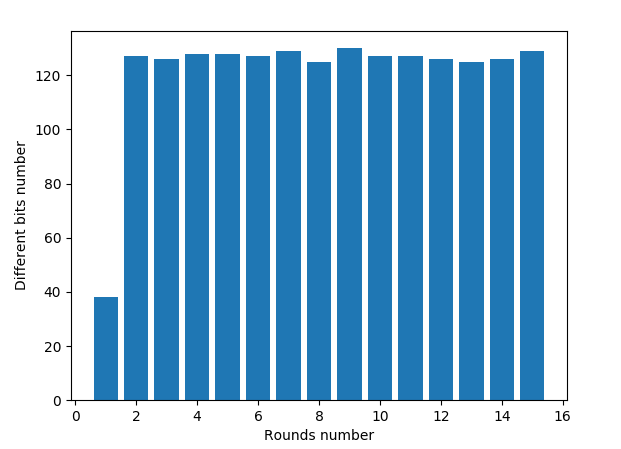
\includegraphics[width=100mm, scale=0.5]{images/bar.png}\\

Такой анализ позволяет увидеть, насколько меняется хеш при минимальном изменении исходного сообщения.
При 256-битном хеше уже со второго раунда меняется половина бит!

\subsection*{Исходный код}
\textbf{da.c}
\lstinputlisting[style=CStyle]{code/da.c}

\subsection*{Консоль}
\begin{lstlisting}
->blake256 ./da
__________________________________
Number of rounds: 1
Number of different bits: 38
__________________________________
Number of rounds: 2
Number of different bits: 127
__________________________________
Number of rounds: 3
Number of different bits: 126
__________________________________
Number of rounds: 4
Number of different bits: 128
__________________________________
Number of rounds: 5
Number of different bits: 128
__________________________________
Number of rounds: 6
Number of different bits: 127
__________________________________
Number of rounds: 7
Number of different bits: 129
__________________________________
Number of rounds: 8
Number of different bits: 125
__________________________________
Number of rounds: 9
Number of different bits: 130
__________________________________
Number of rounds: 10
Number of different bits: 127
__________________________________
Number of rounds: 11
Number of different bits: 127
__________________________________
Number of rounds: 12
Number of different bits: 126
__________________________________
Number of rounds: 13
Number of different bits: 125
__________________________________
Number of rounds: 14
Number of different bits: 126
__________________________________
Number of rounds: 15
Number of different bits: 129

\end{lstlisting}

\newpage

\subsection*{Выводы}
Хеш-функция BLAKE является достаточно криптостойкой, а именно обеспечивает стойкость к атакам второго рода, защиту от коллизий. Алгоритм сжатия является модифицированной версией хорошо параллелизируемого поточного шифра ChaCha, чья безопасность тщательно проанализирована. Интересно, что дифференциальный анализ показал значительные результаты уже на втором раунде, хотя SHA-1 для этого требует, например, не менее 20 раундов, что говорит о явном преимуществе BLAKE. Следует отметить, что на практике используется высокоразвитая версия BLAKE -- BLAKE2, где главным образом улучшено быстродействие.

\end{document}\grid
